
% --------------------------------------Alexandre---------------------------------------------------
%*----------- SLIDE -------------------------------------------------------------
\begin{frame}[c]{O próximo grande marco}
    %\transboxin[duration=1,direction=30]
    Os usos práticos dos AUVs abrangem uma ampla gama.
    \begin{itemize}
        \item exploração subaquática
        \item limpeza de minas
        \item limpeza ou monitaramento de reatores nucleares
    \end{itemize}

    \begin{figure}
        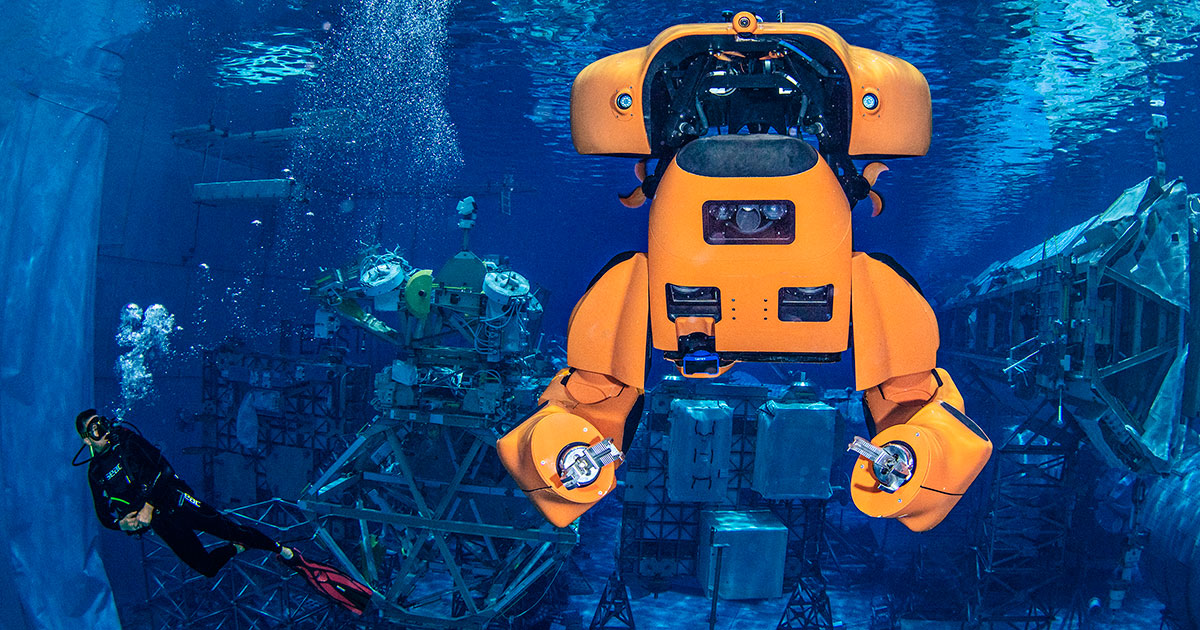
\includegraphics[height = 2.5cm, width=0.3\textwidth]{aquanaut.jpg}
        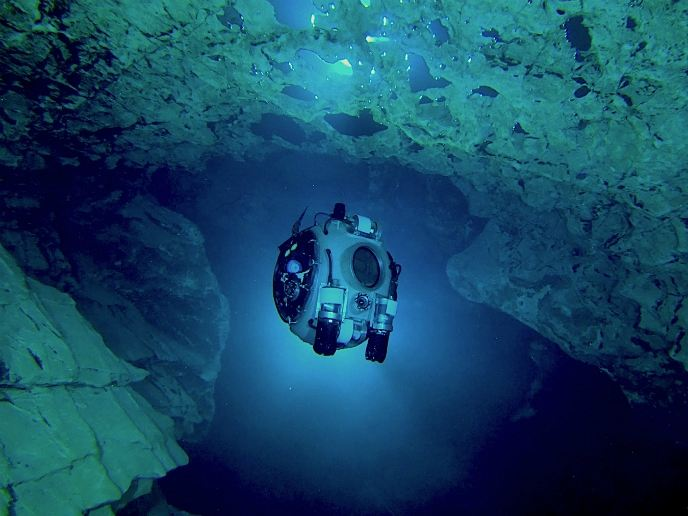
\includegraphics[height = 2.5cm, width=0.3\textwidth]{auv-mines.jpg}
        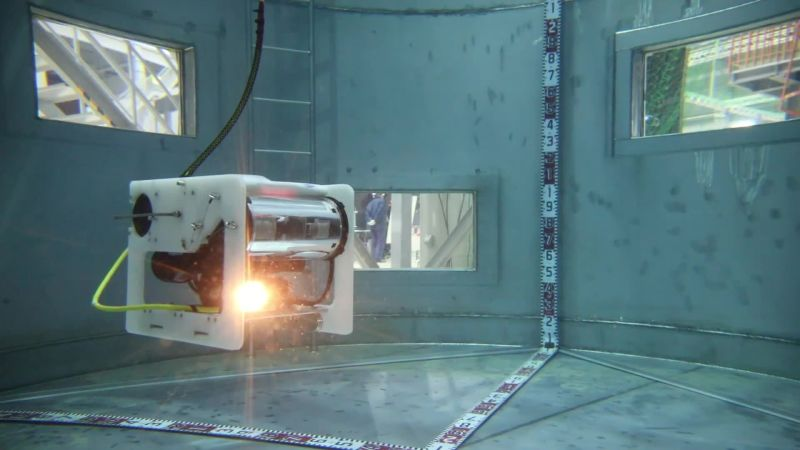
\includegraphics[height = 2.5cm, width=0.3\textwidth]{auv-cleaning.jpg}
        \caption{\nocite{WatchMee87:online}}
        \caption{\nocite{Alookbac39:online}}
        \caption{\nocite{MeetAqua67:online}}
    \end{figure}
%*----------- notes
    \note[item]{Notes can help you to remember important information. Turn on the notes option.}
\end{frame}
%-
%*----------- SLIDE -------------------------------------------------------------
\begin{frame}[c]{Mapa Conceitual}
    %\transboxin[duration=1,direction=30]
        \begin{figure}
        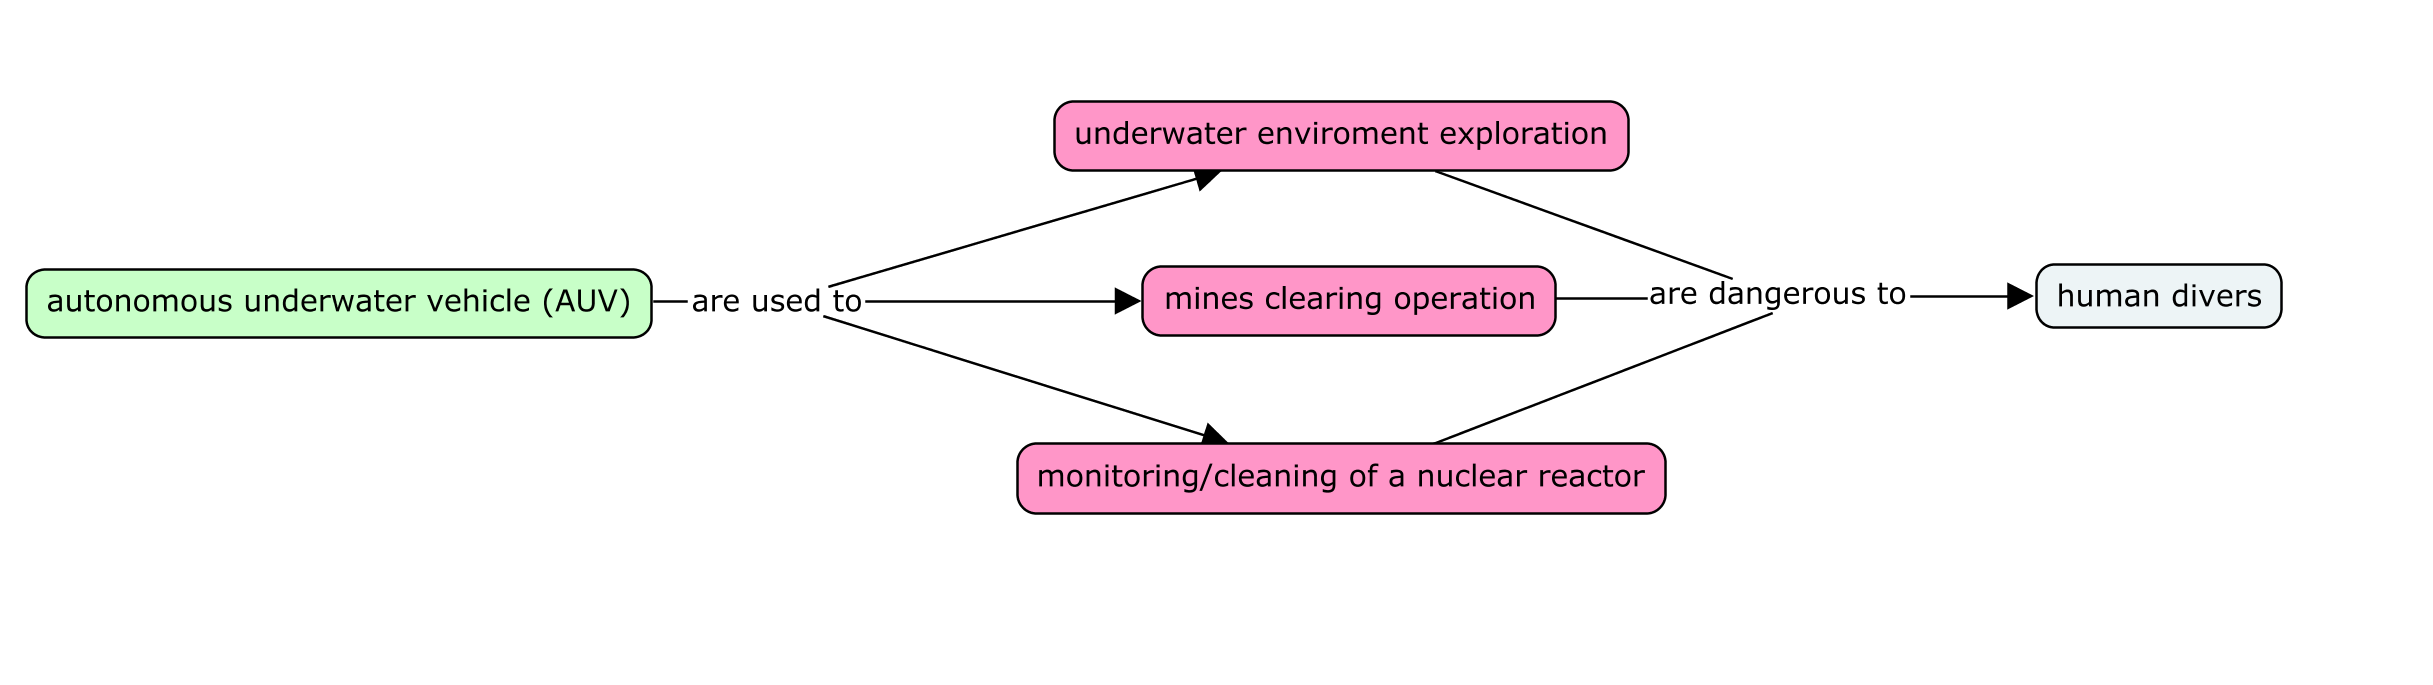
\includegraphics[width=1.1\textwidth]{aplications-map.png}
    \end{figure}
%*----------- notes
    \note[item]{Notes can help you to remember important information. Turn on the notes option.}
\end{frame}
%-
%*----------- SLIDE -------------------------------------------------------------
\begin{frame}[c]{Design}
    %\transboxin[duration=1,direction=30]
    Os AUVs variam em tamanho, sendo eles portáteis até veículos de grande diâmetro.
    \newline
    \begin{columns}[t]
        \column{.05\linewidth}
        
        \column{.4\linewidth}
        \begin{figure}
            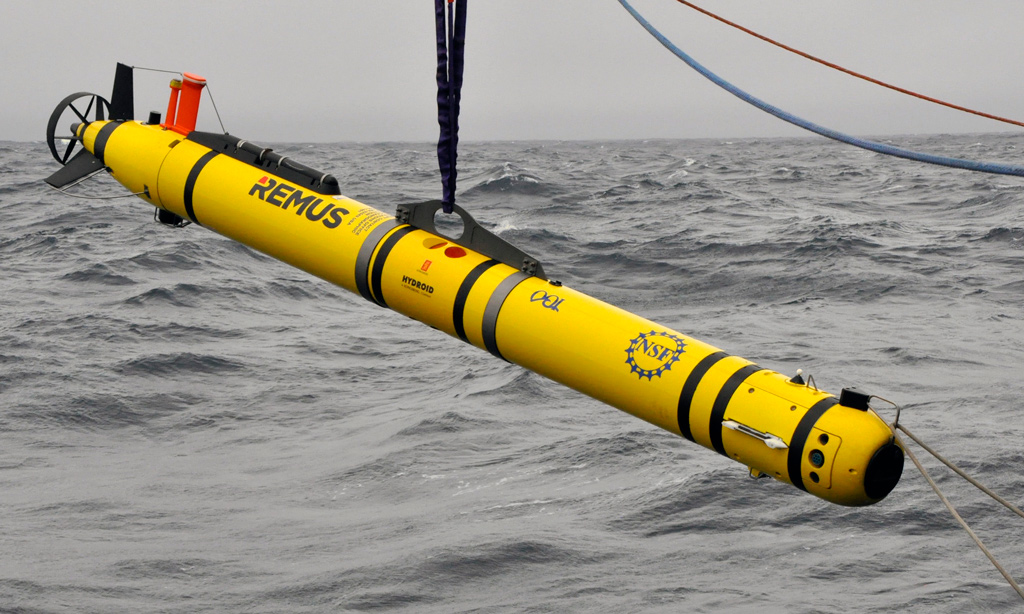
\includegraphics[height = 3.38cm, width=0.8\textwidth]{remus600.jpg}%4.3 metros de comprimento
            \caption{\nocite{REMUS6001:online}}
        \end{figure}
        
        \column{.6\linewidth}
        \begin{figure}
            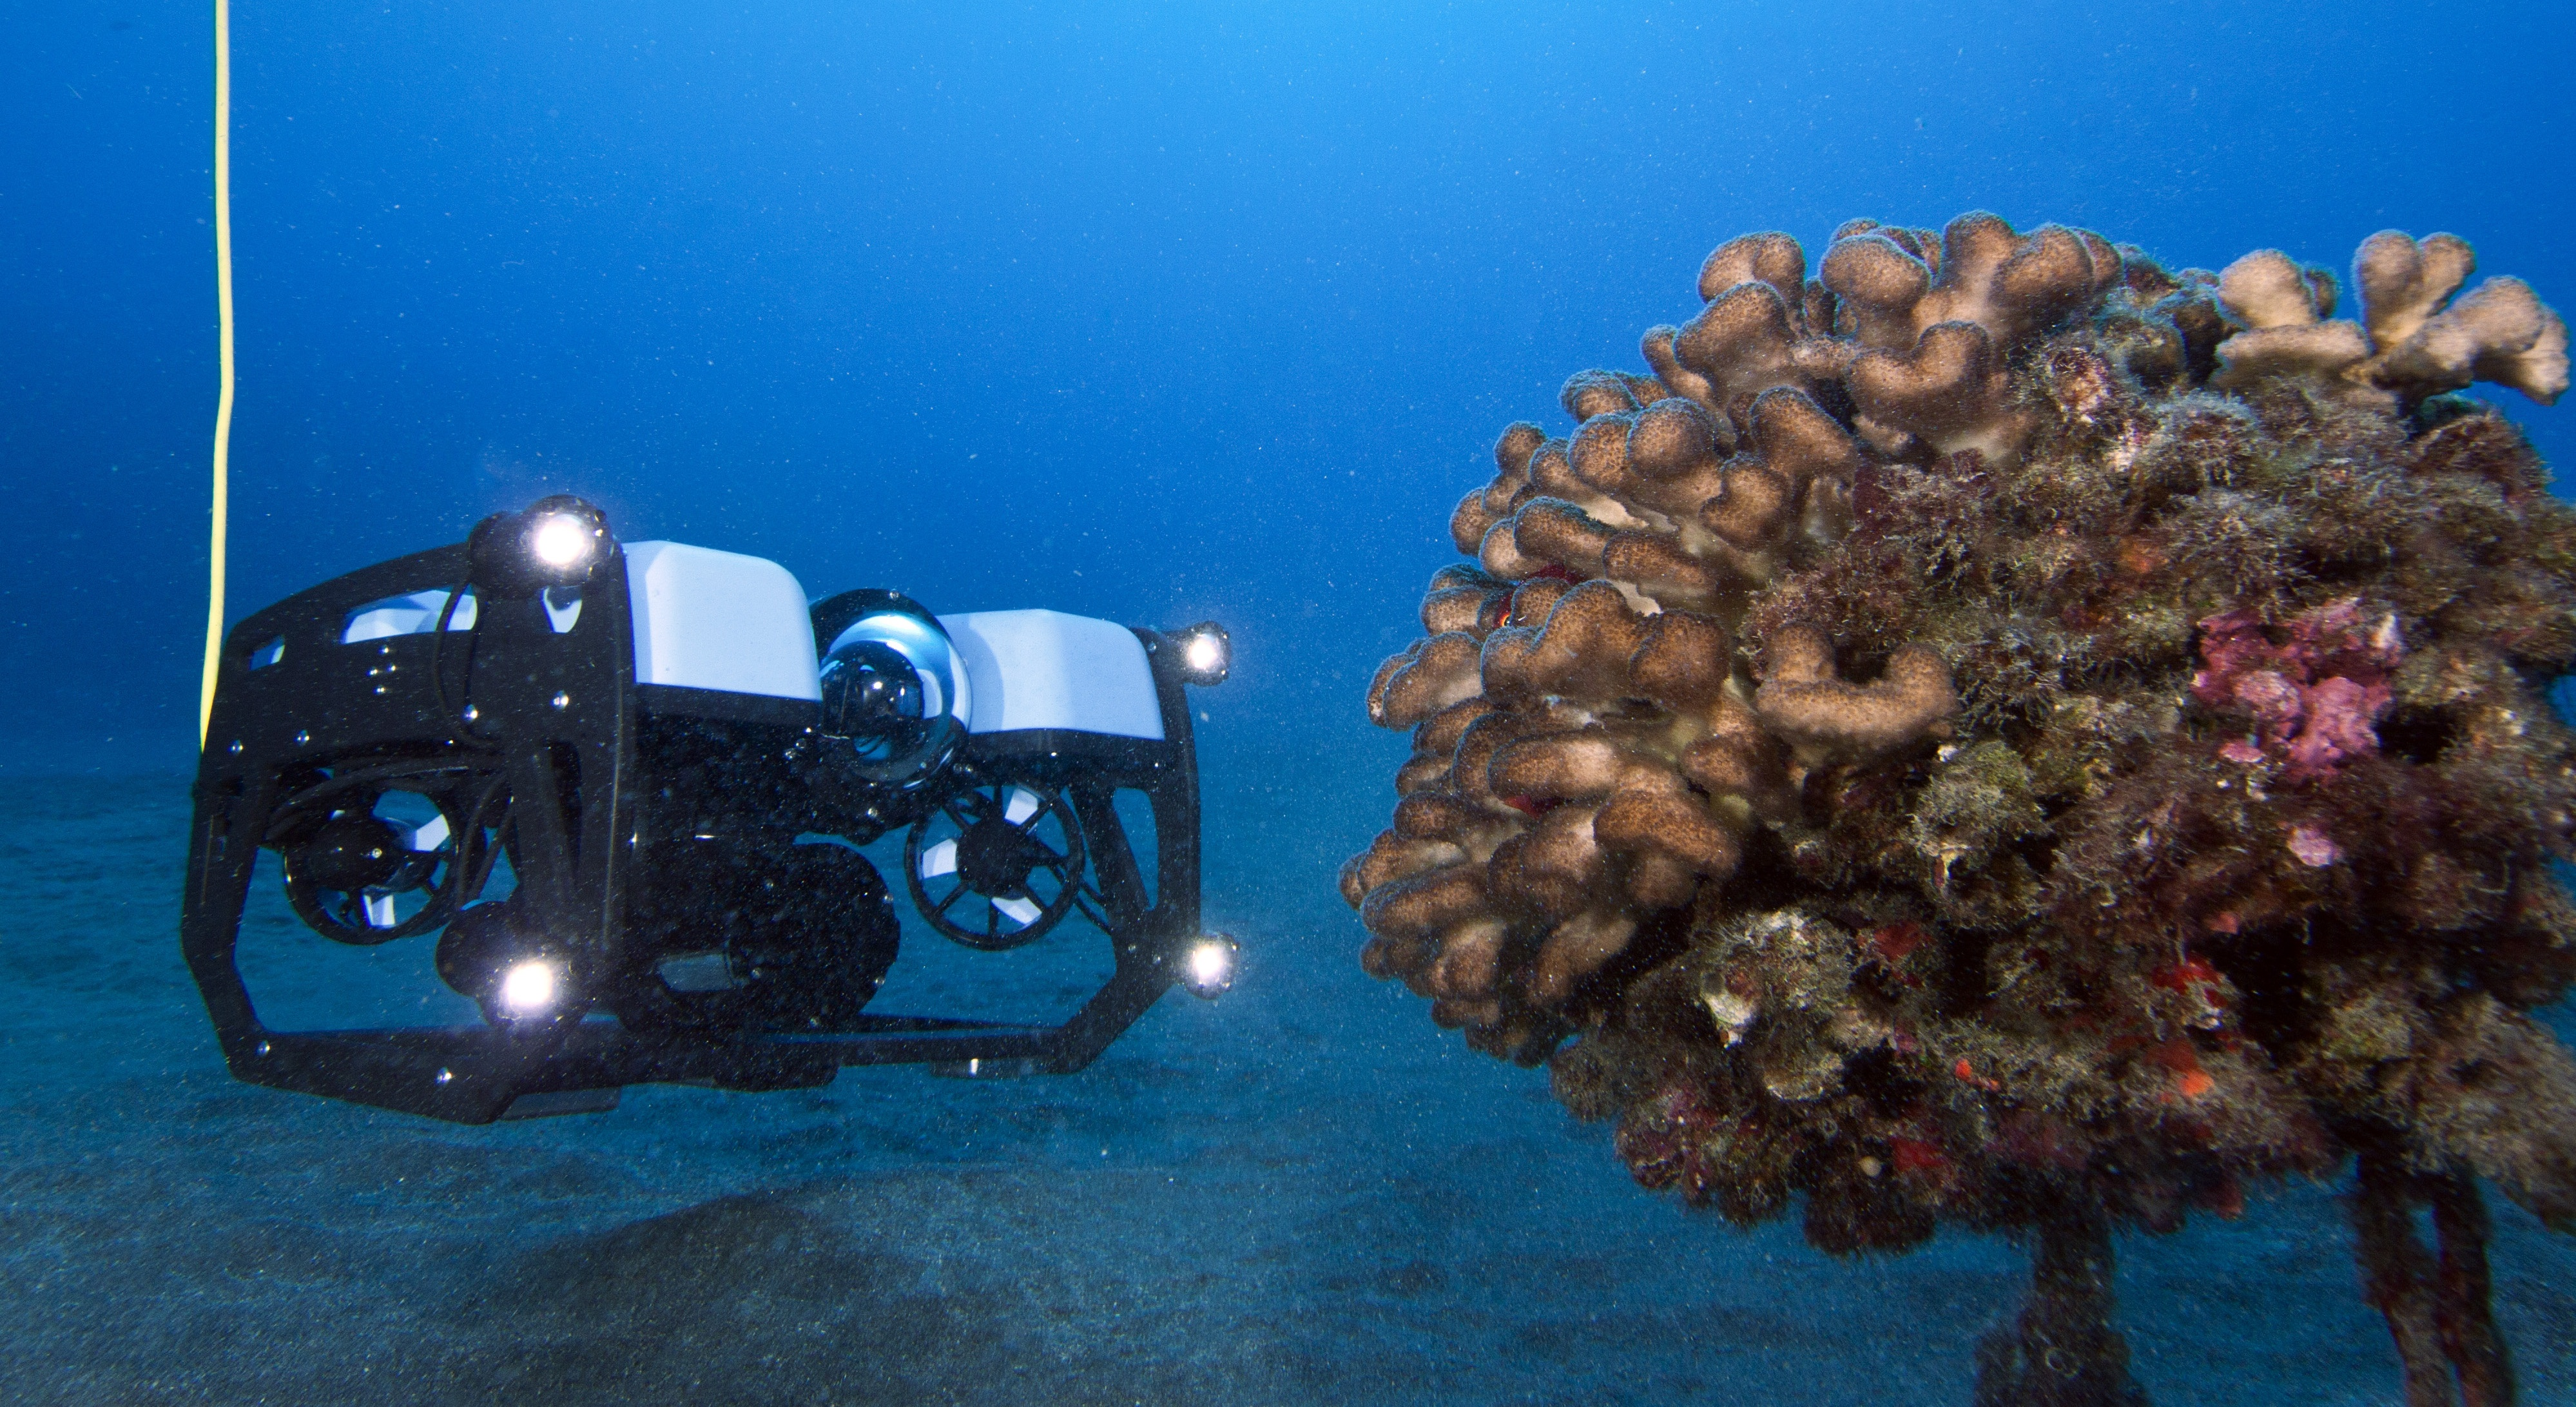
\includegraphics[height = 3.38cm, width=0.6\textwidth]{BlueROV2.jpg}%45.7cm de comprimento
            \caption{\nocite{BlueROV210:online}}
        \end{figure}
        
    \end{columns}
%*----------- notes
    \note[item]{Notes can help you to remember important information. Turn on the notes option.}
\end{frame}
%-
\begin{frame}[c]{Tecnologia AUV}
    %\transboxin[duration=1,direction=30]
    \begin{itemize}
        \item Sistema de Energia
        \item Navegação
        \item Sistema Sensorial
    \end{itemize}

%*----------- notes
    \note[item]{Notes can help you to remember important information. Turn on the notes option.}
\end{frame}

%*----------- SLIDE -------------------------------------------------------------
\begin{frame}[c]{Sistema de Energia}
    %\transboxin[duration=1,direction=30]
    \begin{figure}
        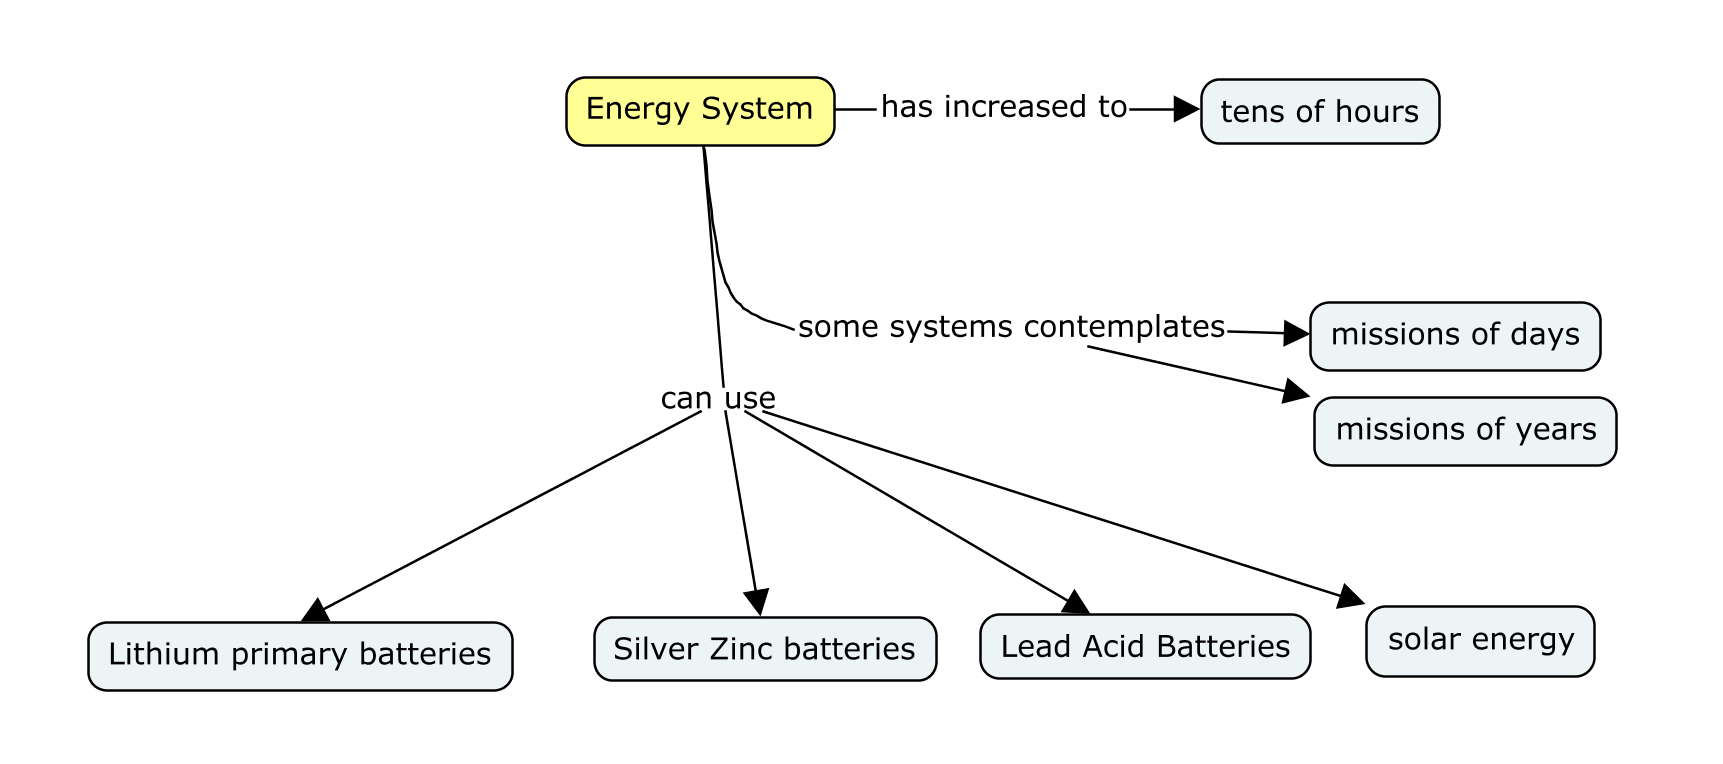
\includegraphics[width=1\textwidth]{energy-system.png}
    \end{figure}
%*----------- notes
    \note[item]{Notes can help you to remember important information. Turn on the notes option.}
\end{frame}
%-

%*----------- SLIDE -------------------------------------------------------------
\begin{frame}[c]{Navegação}
    %\transboxin[duration=1,direction=30]
    \begin{figure}
        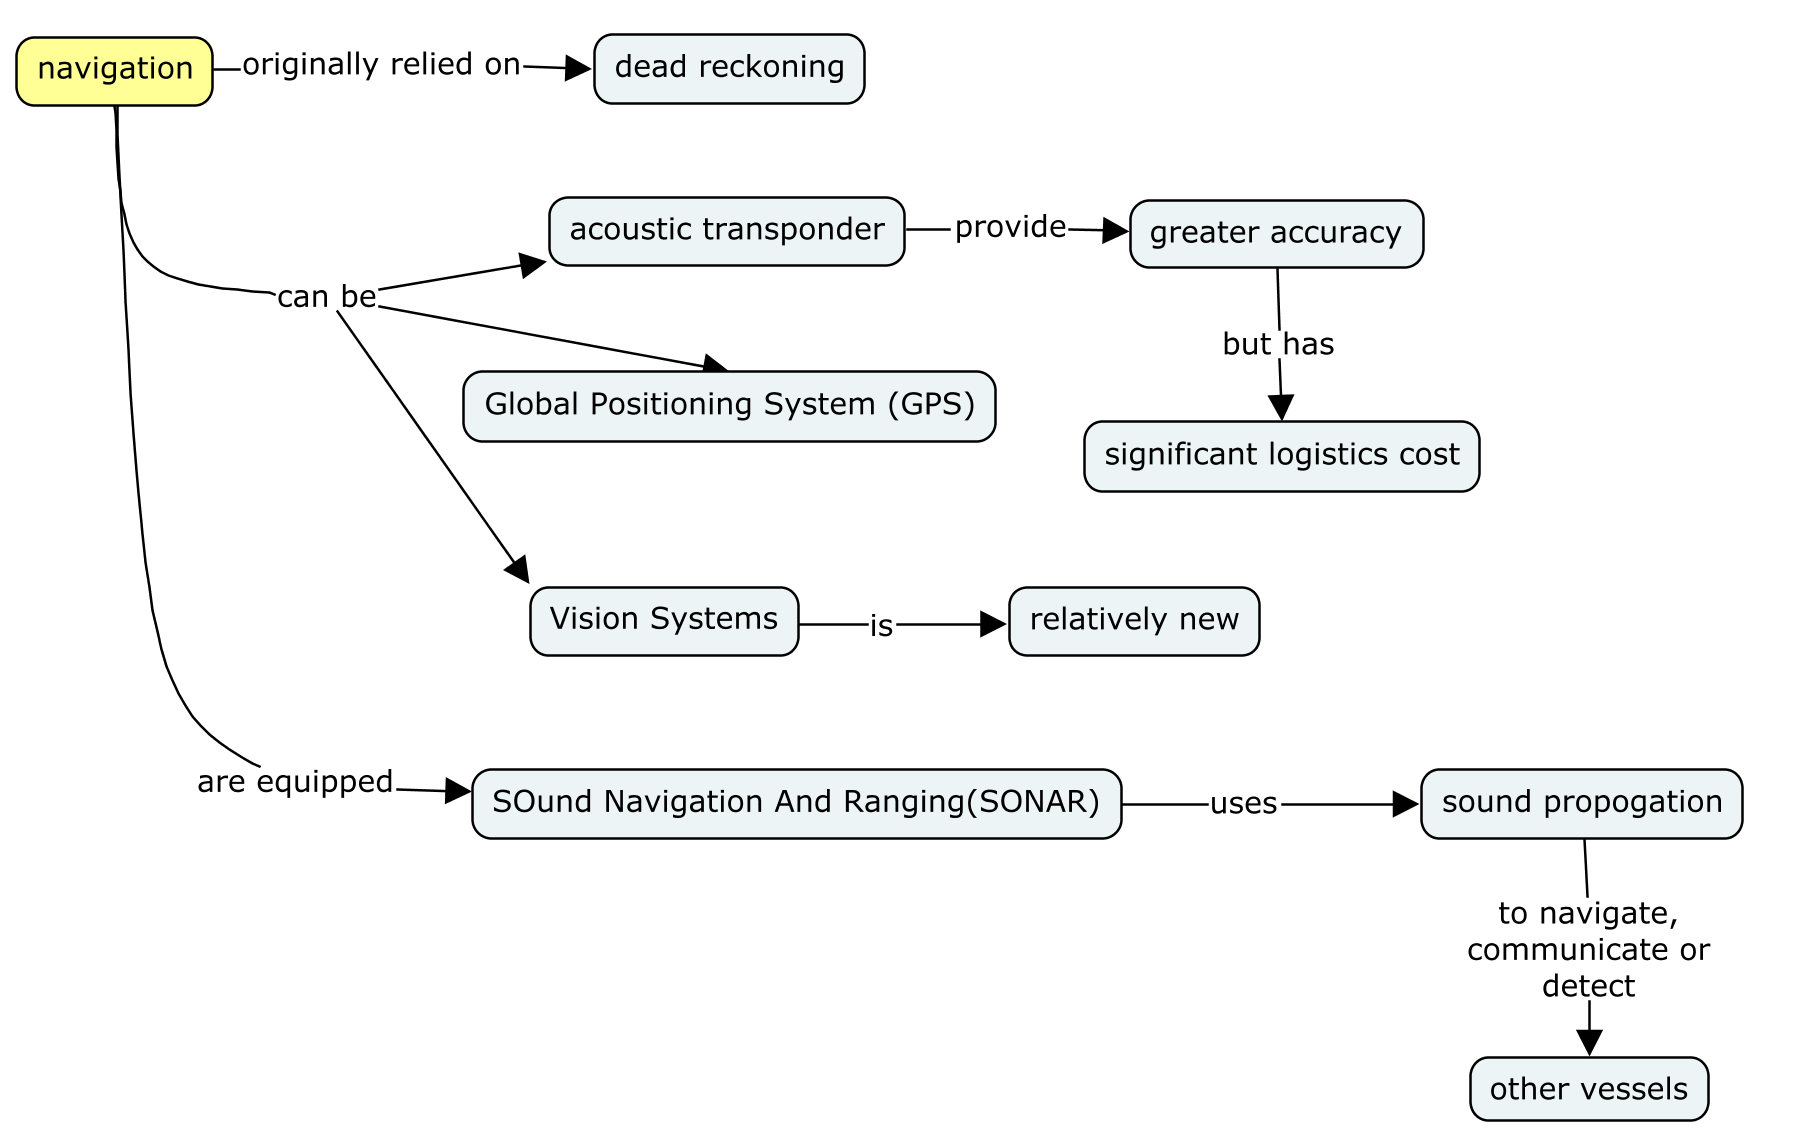
\includegraphics[width=0.77\textwidth]{navigation.png}
    \end{figure}
%*----------- notes
    \note[item]{Notes can help you to remember important information. Turn on the notes option.}
\end{frame}
%-

%*----------- SLIDE -------------------------------------------------------------
\begin{frame}[c]{Sistema Sensorial}
    %\transboxin[duration=1,direction=30]
    \begin{figure}
        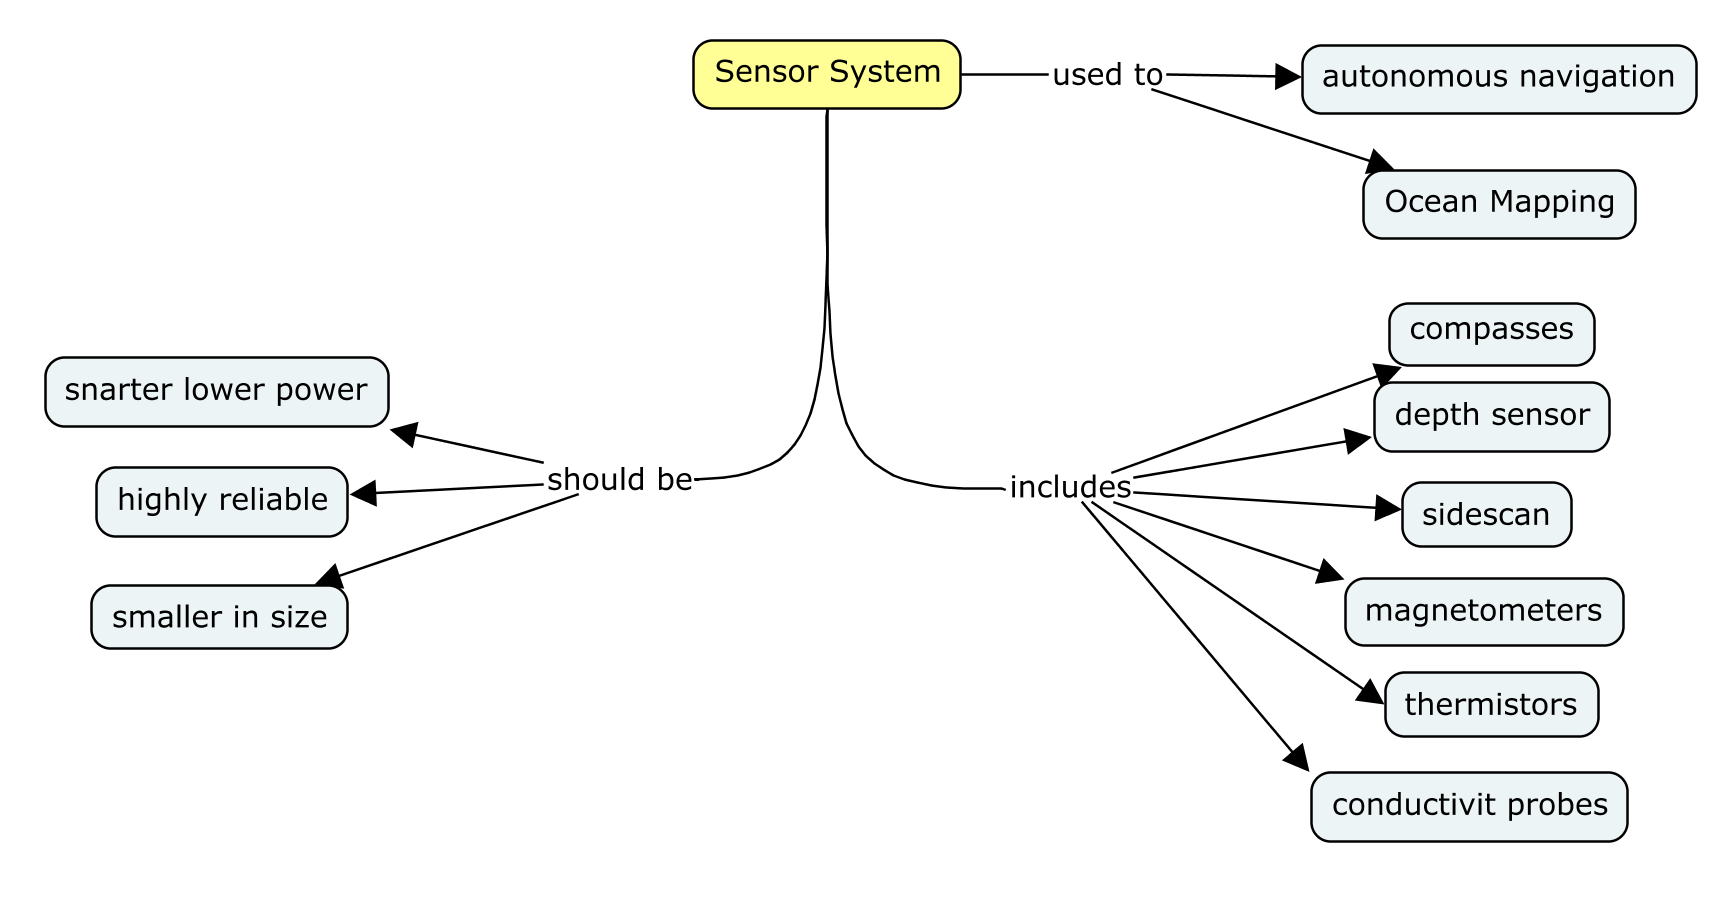
\includegraphics[width=0.95\textwidth]{sensor-system.png}
    \end{figure}
%*----------- notes
    \note[item]{Notes can help you to remember important information. Turn on the notes option.}
\end{frame}
%-